\chapter{Metodología numérica}
\label{C:ap1}
\graphicspath{{figs/}}


El sistema de ecuaciones dado por
\begin{align*}
    \pdv{S}{t}&=-\beta_{\vb{r}} SI + D_{S} \laplacian{S},\\[.3cm]
    \pdv{I}{t}&=\beta_{\vb{r}} SI - \gamma I + D_{I} \laplacian{I},
\end{align*}
se resolvió numéricamente utilizando el siguiente esquema explícito de Euler:

\begin{align*}
    S^{n+1}_{ij} &= S^n_{ij} + \Delta t\left( -\beta_{ij} S^n_{ij}I^n_{ij} + \frac{D_{S}}{d^2} (S^n_{i+1j}+S^n_{i-1j}+S^n_{ij+1}+S^n_{ij-1}-4S^n_{ij})\right)\\[.3cm]
    I^{n+1}_{ij} &= I^n_{ij} + \Delta t\left( \beta_{ij} S^n_{ij}I^n_{ij} - \gamma I^n_{ij} + \frac{D_{I}}{d^2} (I^n_{i+1j}+I^n_{i-1j}+I^n_{ij+1}+I^n_{ij-1}-4I^n_{ij})\right) 
\end{align*}
donde los índices $i$ y $j$ corresponden a la discretización de las coordenadas espaciales y el índice $n$ corresponde a la discretización temporal.
Se utilizaron de manera general los siguientes parámetros $\Delta t=0.1$, $d=1$, $D_{I}=1$ y $D_{S}=0$. Los demás parámetros involucrados se indican 
según corresponde en el texto.

Este esquema se implementó por computación en paralelo utilizando procesadores gráficos. De esta manera fue posible resolver de manera eficiente cientos de sistemas 
sobre grillas de $1024\times1024$. En particular se utilizó la librería de \texttt{Python} para computación en paralelo llamada \texttt{\href{https://cupy.dev/}{CuPy}},
que es un equivalente de la librería \texttt{\href{https://numpy.org/}{NumPy}} pero integrada con \texttt{\href{https://developer.nvidia.com/cuda-toolkit}{CUDA}}.

A continuación se muestra la función central del esquema numérico que permite recorrer la grilla del sistema en paralelo y calcular las derivadas del sistema en 
cada nodo utilizando esta librería, se representan a $S$ e $I$ como $X$ e $Y$ respectivamente:\newpage

\begin{lstlisting}[basicstyle=\tiny]
    forces = cp.ElementwiseKernel(
    'raw float64 X, raw float64 Y, raw float64 params,raw float64 beta,raw float64 gamma, int16 L' ,
    'float64 fX,float64 fY',
    '''
    double N = params[0]; double nu = params[1]; double mu = params[2]; double Dx = params[3];
    double Dy = params[4];
    
    int x = i % L;
    int y = (int) i/L;

    fX =  nu - beta[i]*X[i]*Y[i]/N - mu*X[i] + 
        Dx*(X[(x+1)%L + L*y] + X[(x-1+L)%L+L*y] + X[x + L*((y+1)%L)] + X[x + L*((y-1+L)%L)] - 4*X[i]);

    fY = beta[i]*X[i]*Y[i]/N - (gamma[i]+mu)*Y[i] + 
        Dy*(Y[(x+1)%L + L*y] + Y[(x-1+L)%L+L*y] + Y[x + L*((y+1)%L)] + Y[x + L*((y-1+L)%L)] - 4*Y[i]);
    ''',
    'forces')
\end{lstlisting}

y el paso de Euler se lee simplemente como:

\begin{lstlisting}[basicstyle=\tiny]
    ...
    forces(X,Y,params,beta,gamma,Lx,fX,fY)
    X = X + tstep*fX
    Y = Y + tstep*fY
    ...
\end{lstlisting}

Para dar una idea de la aceleración dada por la programación en paralelo, en la figura \ref{gpuvscpu} se muestra el tiempo necesario para resolver un sistema 
de $N\times N$ sitios y $1000$ pasos de Euler con procesadores gráficos (GPU) y con procesadores convencionales (CPU). La diferencia es notable, por ejemplo, 
para un sistema de $1024\times1024$,
el tiempo necesario para resolverlo con CPU es aproximadamente de 2.7 horas, mientras que con GPU se resuelve en 1 segundo. Se muestra también un ajuste 
para ambas curvas del tipo $t\propto N^a$ con $a\approx2$ para ambos. De todo esto resulta clara la necesidad de trabajar con computación en paralelo 
para obtener los resultados desarrollados en este trabajo en un tiempo razonable. Para ver más detalles acerca del código y 
las herramientas computacionales implementadas puede acceder al siguiente 
\textit{\href{https://colab.research.google.com/drive/1r0242WjJD_a5SR3ppiUQG25x4ODiM4Ps?usp=sharing}{Notebook}} de \textit{Google Colab}.

\begin{figure}[h]
    \centering
    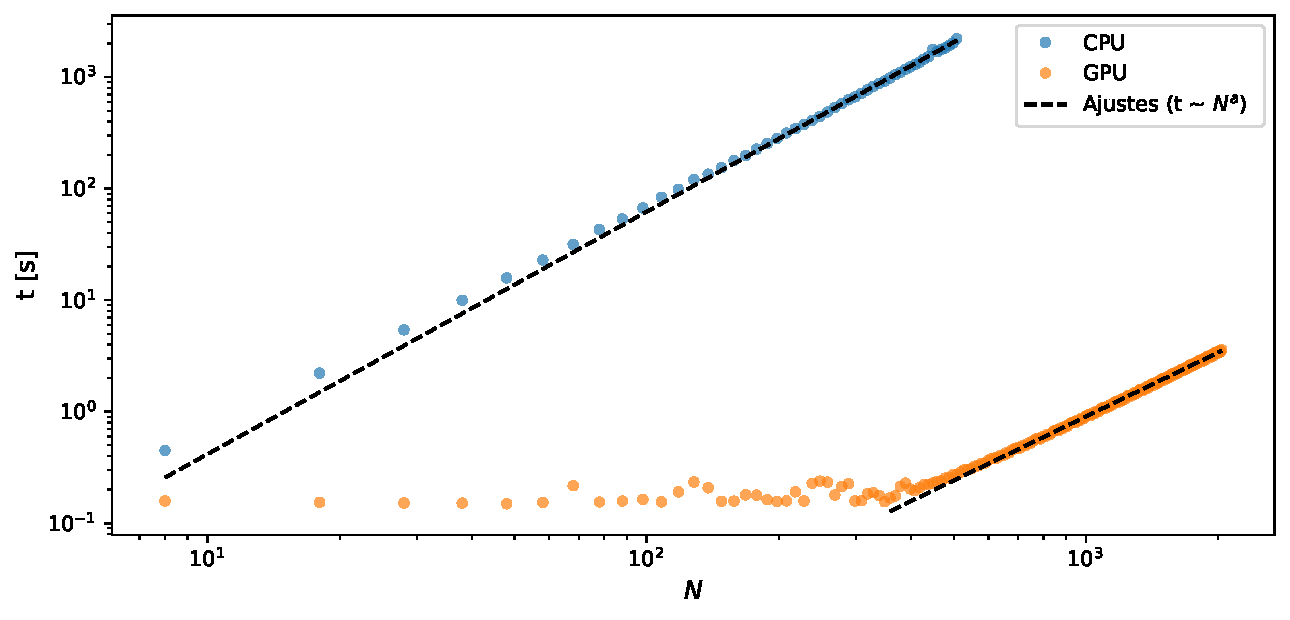
\includegraphics[width=0.8\textwidth]{t_vs_N.pdf}
    \caption{Tiempo de resolución de un sistema de $N\times N$ sitios y 1000 pasos de Euler con procesadores gráficos (GPU) y con procesadores convencionales (CPU). Se muestran 
    también los ajustes de tipo $t\propto N^a$ con $a\approx2$ para ambos.}
    \label{gpuvscpu}
\end{figure}

